\chapter{Theoretische Grundlagen}

Um die Funktionsweise von Augmented Reality (AR) und verwandten Technologien zu verstehen, ist ein grundlegendes Wissen über die zugrunde liegenden Konzepte und Techniken erforderlich. In diesem Kapitel werden die theoretischen Grundlagen der Computer Vision und Computergrafik erläutert, die für die Entwicklung von AR-Anwendungen relevant sind. Dabei wird vor der Fokus vor allem auf die Konzepte gelegt, die eine Relevanz für mobile AR-Anwendungen haben. Dazu gehören die Rekonstruktion von 3D-Szenen, die Kamerakalibrierung, die Sensorik, das Tracking und Rendering von virtuellen Objekten. (\cite{doerner2022virtual})

\section{Dreidimensionale Computergrafik}

In der Computergrafik werden dreidimensionale Objekte, auch als Modelle bezeichnet, durch geometrische und relationale Informationen beschrieben. Diese Objekte bestehen in der Regel aus Polygonen, die durch ihre Eckpunkte (Vertices) definiert sind. Ein Polygon ist eine geschlossene Fläche, die durch das Verbinden der Vertices mit geraden Linien entsteht. Ein 3D-Modell wird in einem kartesischen Koordinatensystem beschrieben, wobei die Positionen der Vertices durch ihre \(x\)-, \(y\)- und \(z\)-Koordinaten angegeben werden. (\cite{kore2018space})

Das einfachste Polygon ist ein Dreieck, das nur drei Eckpunkte benötigt. Dreiecke sind planar und konvex, was sie ideal für Berechnungen in der Computergrafik macht, wie beispielsweise bei der Beleuchtung oder Kollisionserkennung. Obwohl komplexere Polygone existieren, werden diese oft in Dreiecke zerlegt, da sie von Grafikpipelines effizienter verarbeitet werden können. Solche Modelle bestehen dann aus Dreiecksnetzen (Meshes), die als Arrays von Vertices und Indizes gespeichert werden. (\cite{wikipedia2023polygons})

Virtuelle 3D-Szenen und Objekte werden in einem kartesischen Koordinatensystem beschrieben. Dieses Koordinatensystem wird üblicherweise als Weltkoordinatensystem bezeichnet, in dem die \(x\)-, \(y\)- und \(z\)-Achsen die drei Dimensionen repräsentieren. In einem rechtshändigen Koordinatensystem zeigt die \(x\)-Achse nach rechts, die \(y\)-Achse nach oben und die \(z\)-Achse nach vorne. Die Position eines Objekts im Raum wird oft mithilfe einer Transformationsmatrix beschrieben. (\cite{appledevdoc, usau2023appleARCamera})

\section{Matrixalgebra}

Das Anwenden von mathematischen Operationen auf Matrizen ist ein grundlegendes Konzept für viele Algorithmen in der Computer Vision. Diese Arbeit setzt voraus, dass der Leser mit den Grundladen der Matrixalgebra vertraut ist. Im Folgenden werden dennoch die wichtigsten Operationen und Konzepte anhand der Transformationen in der Computergrafik erläutert.

Unter der Transformation eines Objektes in einer 3D-Szene versteht man das Verschieben, Drehen oder Skalieren dieses Objektes. Diese Vorgänge können durch Transformationsmatrizen beschrieben werden, die einheitlich auf alle Vertices eines Objekts angewendet werden. Solche Matrizen haben typischerweise die Größe \(4 \times 4\) und kombinieren Translation, Rotation und Skalierung. Dies hat den Vorteil, dass alle Transformationen in einer einzigen Matrix zusammengefasst werden können, was die Berechnungen effizienter macht. (\cite{jazz2020transformMatrix, pezzi2021matrices, freescale2010math3d})

\subsection{Translation}

Die Translation verschiebt ein Objekt entlang der \(x\)-, \(y\)- oder \(z\)-Achse. Die Transformationsmatrix für eine Translation ist wie folgt definiert:

\begin{equation}
\begin{bmatrix}
x' \\ y' \\ z' \\ 1
\end{bmatrix}
=
\begin{bmatrix}
1 & 0 & 0 & t_x \\
0 & 1 & 0 & t_y \\
0 & 0 & 1 & t_z \\
0 & 0 & 0 & 1
\end{bmatrix}
\begin{bmatrix}
x \\ y \\ z \\ 1
\end{bmatrix}
\end{equation}

Hierbei verschieben die Parameter \(t_x\), \(t_y\) und \(t_z\) das Objekt entlang der jeweiligen Achsen.

\subsection{Rotation}

Die Rotation eines Objekts erfolgt um eine der drei Achsen. Die Rotationsmatrizen sind für jede Achse wie folgt definiert:

\paragraph{Rotation um die \(x\)-Achse:}
\begin{equation}
\begin{bmatrix}
1 & 0 & 0 & 0 \\
0 & \cos(\alpha) & -\sin(\alpha) & 0 \\
0 & \sin(\alpha) & \cos(\alpha) & 0 \\
0 & 0 & 0 & 1
\end{bmatrix}
\end{equation}

\paragraph{Rotation um die \(y\)-Achse:}
\begin{equation}
\begin{bmatrix}
\cos(\alpha) & 0 & \sin(\alpha) & 0 \\
0 & 1 & 0 & 0 \\
-\sin(\alpha) & 0 & \cos(\alpha) & 0 \\
0 & 0 & 0 & 1
\end{bmatrix}
\end{equation}

\paragraph{Rotation um die \(z\)-Achse:}
\begin{equation}
\begin{bmatrix}
\cos(\alpha) & -\sin(\alpha) & 0 & 0 \\
\sin(\alpha) & \cos(\alpha) & 0 & 0 \\
0 & 0 & 1 & 0 \\
0 & 0 & 0 & 1
\end{bmatrix}
\end{equation}

Die Reihenfolge, in der Rotationen um verschiedene Achsen durchgeführt werden, ist entscheidend, da sie die finale Orientierung und Position des Objektes beeinflussen. Diese Reihenfolge wird durch Euler-Winkel beschrieben.

\subsection{Skalierung}

Die Skalierung verändert die Größe eines Objekts proportional entlang der \(x\)-, \(y\)- und \(z\)-Achsen. Die Skalierungsmatrix ist wie folgt definiert:

\begin{equation}
\begin{bmatrix}
x' \\ y' \\ z' \\ 1
\end{bmatrix}
=
\begin{bmatrix}
s_x & 0 & 0 & 0 \\
0 & s_y & 0 & 0 \\
0 & 0 & s_z & 0 \\
0 & 0 & 0 & 1
\end{bmatrix}
\begin{bmatrix}
x \\ y \\ z \\ 1
\end{bmatrix}
\end{equation}

Hierbei sind \(s_x\), \(s_y\) und \(s_z\) die Skalierungsfaktoren entlang der jeweiligen Achsen.

\subsection{Anwendung der Transformationen}

Die lokalen Koordinaten eines Objekts können mithilfe einer Transformationsmatrix in Weltkoordinaten umgerechnet werden:

\begin{equation}
P_{world} = T_{object} \cdot P_{object}
\end{equation}

Hierbei ist \(T_{object}\) die Transformationsmatrix des Objekts, und \(P_{object}\) sind die lokalen Koordinaten. Das Ergebnis \(P_{world}\) beschreibt die Position des Objekts im Weltkoordinatensystem.

\section{Kalibrierung}\label{Kalibrierung}

Die Kalibrierung ist ein essenzieller Schritt in der Augmented-Reality-Pipeline. Sie dient der Bestimmung der intrinsischen und extrinsischen Kameraparameter, um eine korrekte Transformation von 2D-Bildpunkten in 3D-Weltkoordinaten zu ermöglichen (\cite{mw2024calibration}).

Dabei wird häufig das sogenannte „Pinhole“-Modell verwendet, das die grundlegenden Eigenschaften einer idealisierten Kamera beschreibt (siehe Abbildung \ref{fig:Pinhole}). Dieses Modell basiert auf der Annahme einer Kamera ohne Objektiv, die lediglich eine kleine Blendenöffnung besitzt. Das Licht fällt durch diese Blende und projiziert ein umgekehrtes Abbild der Szene auf die Rückwand der Kamera (\cite{mw2024calibration}).

\begin{figure}
    \centering
    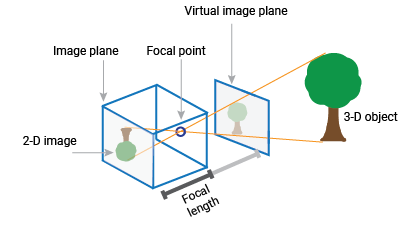
\includegraphics[ width=.5\textwidth ]{pinhole}
    \caption{Pinhole-Modell (\cite{mw2024calibration})\label{fig:Pinhole}}\par
\end{figure}

Mithilfe der intrinsischen und extrinsischen Parameter kann eine Projektionsmatrix bestimmt werden, die es ermöglicht, Bildpixel in das Koordinatensystem der realen Welt zu überführen (siehe Abbildung \ref{fig:Kalibrierung}). Die intrinsischen Parameter umfassen die Brennweite, die Objektivverzerrung und die Position des optischen Zentrums der Kamera. Die extrinsischen Parameter hingegen beschreiben die Position und Orientierung der Kamera im Raum (\cite{mw2024calibration}).

\begin{figure}
    \centering
    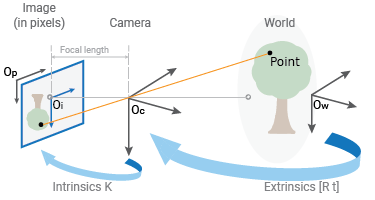
\includegraphics[ width=.5\textwidth ]{calibration-cameramodel-coords}
    \caption{Modell für die Kamerakalibrierung (\cite{mw2024calibration})\label{fig:Kalibrierung}}\par
\end{figure}

Mathematisch wird die Projektionsmatrix \(P\) wie folgt definiert (\cite{mw2024calibration, szeliski2022computerVision}):

\[
P = K[R|t]
\]

Hierbei entspricht \(K\) der intrinsischen Matrix. \(R\) die Rotationsmatrix und \(t\) der Translationsvektor der extrinsischen Matrix. Die intrinsische Matrix \(K\) ist definiert als (\cite{mw2024calibration}):

\[
K = 
\begin{bmatrix}
f_x & s & c_x \\
0 & f_y & c_y \\
0 & 0 & 1
\end{bmatrix}
\]

Hier gilt:

\begin{itemize}
    \item \( f_x \) und \( f_y \): Brennweiten der Kamera in Pixeln, bezogen auf die horizontalen und vertikalen Achsen.
    \item \( c_x \) und \( c_y \): Koordinaten des optischen Zentrums in Pixeln.
    \item \( s \): Skew-Faktor, der berücksichtigt, ob die Kameraachsen orthogonal sind.
\end{itemize}

Die Projektion eines 3D-Punktes \( X = [X, Y, Z, 1]^T \) in das Bildkoordinatensystem \( x = [x, y, 1]^T \) erfolgt dann durch die Gleichung (\cite{mw2024calibration}):

\[
x = PX
\]

Ein Bestandteil der intrinsischen Parameter, das gesondert betrachtet werden muss, sind die Verzerrungen der Linse (engl. Lens-Distortions). Diese entstehen zum einen durch die Krümmung der Linse (Radiale Verzerrzng) und zum anderen durch Unterschiede der Ausrichtung der Linse und des Sensors (Tangentiale Verzerrung). Ohne diese Verzerrungen in die Berechnungen einzubeziehen, kann es Unstimmigkeiten zwischen den berechneten Weltkoordinaten und den realen Weltkoordinaten für einen Bildpunkt geben (\cite{mw2024calibration, szeliski2022computerVision}).

Dazu werden oft Polynommodelle, wie das Brown-Conrady-Modell, verwendet. Dieses Modell relative Position zwischen der Linse und des Sensors. die radiale und tangentialen Verzerrungen der Linse und wird durch die Koeffizienten \( k_1, k_2, k_3 \) und \( p_1, p_2 \) definiert (\cite{brown1966distortion}). Die radiale Verzerrung kann somit durch folgende Gleichung beschrieben werden (\cite{mw2024calibration, szeliski2022computerVision}):

\[
x_{\text{distorted}}   
=
x_{\text{undistorted}}
\left( 1 + k_1 r^2 + k_2 r^4 + k_3 r^6 \right)
\]
\[
y_{\text{distorted}}   
=
y_{\text{undistorted}}
\left( 1 + k_1 r^2 + k_2 r^4 + k_3 r^6 \right)
\]

In diesem Kapitel wurde die Kamera-Kalibrierung anhand einfacher Modelle erläutert. In der Praxis sind die intrinsischen Parameter jedoch in den meisten Kameras bereits vorkalibriert und können von den Herstellern bereitgestellt werden. So integriert beispielsweise Apples ARKit die intrinsischen Kameraparameter direkt und stellt sie über die Klasse \texttt{AVCameraCalibrationData} zur Verfügung, wodurch sie einfach genutzt werden können (\cite{appledevdoc}).

Die extrinsischen Parameter hingegen müssen häufig manuell bestimmt werden, um die exakte Position und Orientierung der Kamera zu ermitteln. In der Augmented Reality ist die präzise Bestimmung der Kameraposition essenziell für viele Tracking-Verfahren. Dabei unterscheidet man zwischen markerbasiertem Tracking (siehe Kapitel \ref{Markerbasiertes Tracking}), bei dem die Position und Größe eines bekannten Markers – oft ein Schachbrettmuster – in der realen Welt genutzt wird, und markerlosem Tracking (siehe Kapitel \ref{SfM} und \ref{SLAM}), bei dem die Kameraposition durch die Analyse von Bilddaten ermittelt wird (\cite{doerner2022virtual, alam2024calibration}).

\section{Sensorik}

Die Erfassung der Umgebung in Augmented-Reality-Anwendungen erfolgt mithilfe verschiedener Sensoren, die Daten über die physische Welt liefern. Je nach Anwendungsfall und Eingabegerät können unterschiedliche Sensoren verwendet werden, um die Position und Bewegung des Geräts zu bestimmen. Bei vielen Tracking-Verfahren werden eine Kombination von Sensoren verwendet, um die Genauigkeit und Zuverlässigkeit der Positionsschätzung zu verbessern. Beispielsweise kann die Kamera für visuelle Tracking-Anwendungen verwendet werden, während das IMU für die Schätzung der Bewegung des Geräts verwendet wird. Durch die Fusion von Daten aus verschiedenen Sensoren können AR-Anwendungen eine präzise und konsistente Darstellung der virtuellen Objekte in der realen Welt erreichen. Die wichtigsten Sensorenarten werden in diesem Abschnitt erläutert.

\subsection{Inertiale Sensoren}

Inertiale Sensoren erfassen die Beschleunigung und Rotation eines Geräts und bestehen typischerweise aus einem Gyroskop und einem Beschleunigungsmesser. Während das Gyroskop die Winkelgeschwindigkeit misst und Drehbewegungen erkennt, erfasst der Beschleunigungsmesser lineare Beschleunigungen. Durch die Kombination beider Sensoren in einer Inertial Measurement Unit (IMU) lassen sich Bewegungen in sechs Freiheitsgraden (3D-Position und -Orientierung) präzise bestimmen. Diese Technologie ist besonders nützlich zur Erfassung schneller Bewegungen und findet Anwendung in AR-Brillen, Smartphones und anderen mobilen Geräten (\cite{doerner2022virtual}).

\begin{tcolorbox}[colback=THAi-Blue!20!white, colframe=THAi-Blue]
    Als \textbf{Freiheitsgrade} (engl. Degrees of Freedom – DOF) werden voneinander unabhängige Bewegungsmöglichkeiten eines physikalischen Systems bezeichnet. Ein starrer Körper besitzt sechs Freiheitsgrade: je drei für die Translation und Rotation. //TODO: Quelle
\end{tcolorbox}
    

\subsection{Kamera}

Die Kamera ist ein essentieller Sensor für AR-Anwendungen, da die visuellen Informationen von vielen Tracking-Verfahren genutzt werden und die aufgenommenen Bilder die Grundlage für die Darstellung von virtuellen Objekten in der realen Welt bilden. Die Kamera liefert Bilddaten, die zur Erkennung von Markern, Features oder Objekten verwendet werden. Durch die Analyse der Kamerabilder können AR-Anwendungen die Position und Orientierung des Geräts bestimmen und virtuelle Objekte in die reale Welt einfügen. (\cite{doerner2022virtual}).

\subsection{Lasersensoren}

Lasersensoren messen die Entfernung zu Objekten mithilfe von Laserstrahlen. LiDAR (Light Detection and Ranging) ist ein bekannter Lasersensor, der in der Robotik, Automobilindustrie und Augmented Reality weit verbreitet ist. Der Sensor strahlt Laserlicht aus und misst die Zeit, die das Licht benötigt, um zu einem Punkt in der Umgebung zu gelangen und zurückzukehren. Dadurch ist die exakte Bestimmung der Position und Entfernung des Punktes zum Sensor möglich. Dies ermöglicht die präzise Erfassung von Tiefeninformationen in der Umgebung und bietet somit große Vorteile für die Genauigkeit und Zuverlässigkeit des Trackings in AR-Anwendungen (\cite{doerner2022virtual}).

\subsection{Satellitengestütze Systeme}

Satellitengestützte Systeme wie GPS (Global Positioning System) bestimmen die geografische Position des Geräts mithilfe von Satellitensignalen. Diese Systeme sind besonders nützlich für die Lokalisierung des Geräts in großen Außenbereichen. Da GPS-Signale jedoch durch Gebäude und andere Hindernisse blockiert werden können, sind sie in Innenräumen oft ungenau. Zusätzlich dazu sind Abweichungen von bis zu 10m möglich, was für viele AR-Anwendungen nicht ausreichend ist. Smartphones setzen daher häufig A-GPS (Assisted GPS) ein um die GPS-Daten mithilfe von Mobilfunknetz- bzw. WLAN-Daten zu präzisieren (\cite{doerner2022virtual}). 

\subsection{Magnetfeldbasierte Sensoren}

Magnetfeldbasierte Sensoren, wie das Magnetometer in IMUs, messen das Magnetfeld der Erde und liefern so Rückschlüsse bezüglich der Orientierung des Geräts relativ zum Magnetfeld. Diese Sensoren sind besonders nützlich für die Bestimmung der Ausrichtung des Geräts im Raum. Allerdings sind Magnetfelder anfällig für Störungen durch elektrische Geräte und Metallgegenstände, was die Genauigkeit der Messungen beeinträchtigen kann. Dennoch sind magnetfeldbasierte Sensoren eine wichtige Ergänzung zu anderen Sensoren für die präzise Lokalisierung und Orientierung in AR-Anwendungen (\cite{doerner2022virtual}).

\section{Markenbasiertes Tracking}\label{Markerbasiertes Tracking}

Das markenbasierte Tracking nutzt spezielle Marker, die in der realen Welt platziert werden und als Referenzpunkte für die Positionierung virtueller Objekte dienen. Diese Marker ermöglichen die Bestimmung der extrinsischen Kameraparameter und weisen in der Regel ein eindeutiges Muster auf, das von der Kamera erkannt und verfolgt wird. Da die Dimensionen des Markers bekannt sind, kann seine Position und Orientierung im Raum präzise berechnet werden. Es gibt verschiedene Verfahren, die unterschiedliche Marker-Typen verwenden und jeweils eigene Methoden zur Positions- und Orientierungsbestimmung nutzen. (\cite{doerner2022virtual}) 

Vereinfacht dargestellt, funktioniert das markenbasierte Tracking wie folgt:

\begin{figure}
    \centering
    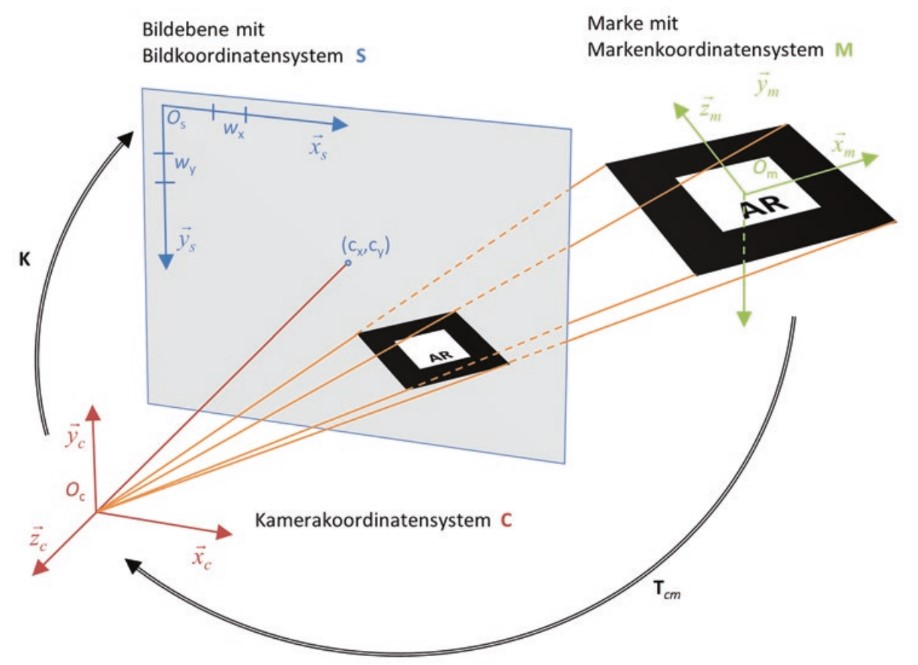
\includegraphics[ width=.5\textwidth ]{Marker}
    \caption{Darstellung eines markenbasiertes Tracking\label{fig:Marker}}\par
\end{figure}

Wie in Abbildung \ref{fig:Marker} dargestellt, wird die Kamera auf den Marker ausgerichtet, um ihn zu erfassen. Anhand der intrinsischen Kameraparameter und der bekannten Abmessungen des Markers lässt sich die Position und Orientierung des Kamerakoordinatensystems \( S \) relativ zum Marker bestimmen. Dadurch kann die Transformationsmatrix \( T_{cm} \) berechnet werden, mit der die Koordinaten des Markers aus dem Markerkoordinatensystem in das Kamerakoordinatensystem überführt werden. (\cite{doerner2022virtual})

Entsprechend der Abbildung \ref{fig:Marker} lässt sich die Transformation \( T_{cm} \) wie folgt definieren:

\begin{equation}\label{eq:v_c}
    v_c = T_{cm} * v_m
\end{equation}

Dabei bezeichnet \( v_c \) Koordinaten im Kamerakoordinatensystem, während \( v_m \) Koordinaten im Markerkoordinatensystem darstellen (\cite{doerner2022virtual}).  

Die Koordinaten \( v_s \) im Bildkoordinatensystem \( C \) lassen sich unter Verwendung der intrinsischen Kameraparameter (siehe Kapitel \ref{Kalibrierung}) sowie der Koordinaten \( v_c \) im Kamerakoordinatensystem wie folgt ausdrücken (\cite{doerner2022virtual}):


\begin{equation}
    v_s = K * v_c
\end{equation}

Unter Verwendung der Gleichung \ref{eq:v_c} kann die Transformation \( T_{cm} \) in die Gleichung eingesetzt werden:

\begin{equation}
    v_s = K * T_{cm} * v_m
\end{equation}

Da sowohl \( v_s \) als auch \( v_m \) bekannt sind, also die Pixelkoordinaten des Markers und seine realen Abmessungen, lässt sich die Transformationsmatrix \( T_{cm} \) bestimmen. Diese entspricht der extrinsischen Kameramatrix \( [R|t] \), welche die Position und Orientierung der Kamera relativ zum Marker beschreibt. Die berechnete Transformation kann anschließend zur präzisen Platzierung virtueller Objekte genutzt werden. (\cite{doerner2022virtual}) 


//TODO: Berechnung der Transformationsmatrix

Das markenbasierte Tracking zeichnet sich durch hohe Präzision und Robustheit aus. Deshalb wird diese Methode häufig in Anwendungen eingesetzt, bei denen die exakte Position des darzustellenden Objekts im Vorfeld bekannt ist. Allerdings ist das markenbasierte Tracking auf die Verwendung von speziellen Markern beschränkt, was die Flexibilität und Anwendbarkeit in verschiedenen Szenarien einschränken kann. Daher werden zunehmend markerlose Tracking-Verfahren bevorzugt, die ohne spezielle Marker auskommen und die Kameraposition anhand von Bildinformationen schätzen. Diese Verfahren werden im folgenden Abschnitt erläutert. (\cite{doerner2022virtual})

\section{SLAM}\label{SLAM}

Simultanous Localization and Mapping (SLAM) hat sich als eine der wichtigsten Technologien in der Augmented Reality etabliert. Das Verfahren, das ursprünglich aus der Robotik stammt, ermöglicht die gleichzeitige Bestimmung der Position und Orientierung eines Geräts und die Extraktion dreidimensionaler Informationen der Umgebung. SLAM wird in einer Vielzahl von AR-Framworks und -Anwendung eingesetzt.


SLAM ermöglicht es, die Position und Orientierung eines Geräts in Echtzeit zu bestimmen und gleichzeitig eine Karte der Umgebung zu erstellen. Diese Technologie ist besonders nützlich für mobile AR-Anwendungen, da sie eine präzise Lokalisierung und Orientierung des Geräts in der realen Welt ermöglicht. SLAM wird in einer Vielzahl von Anwendungen eingesetzt, wie beispielsweise in der Navigation, der Robotik und der Augmented Reality. (\cite{doerner2022virtual})

Simultanous Localization and Mapping (SLAM) entstammt urprünglich aus der Robotik und beschreibt die Fähigkeit eines autonomen Systems, sich in einer unbekannten Umgebung zu lokalisieren und gleichzeitig eine Karte dieser Umgebung zu erstellen. SLAM wird in einer Vielzahl von mobile AR-Anwendung und Frameworks eingesetzt. Dort tritt es oft in Form des Visual SLAM auf, bei dem sowohl visuelle Informationen der Kamera als auch Informationen anderer Sensoren, wie IMUs oder LiDAR, genutzt werden. 

\begin{figure}
    \centering
    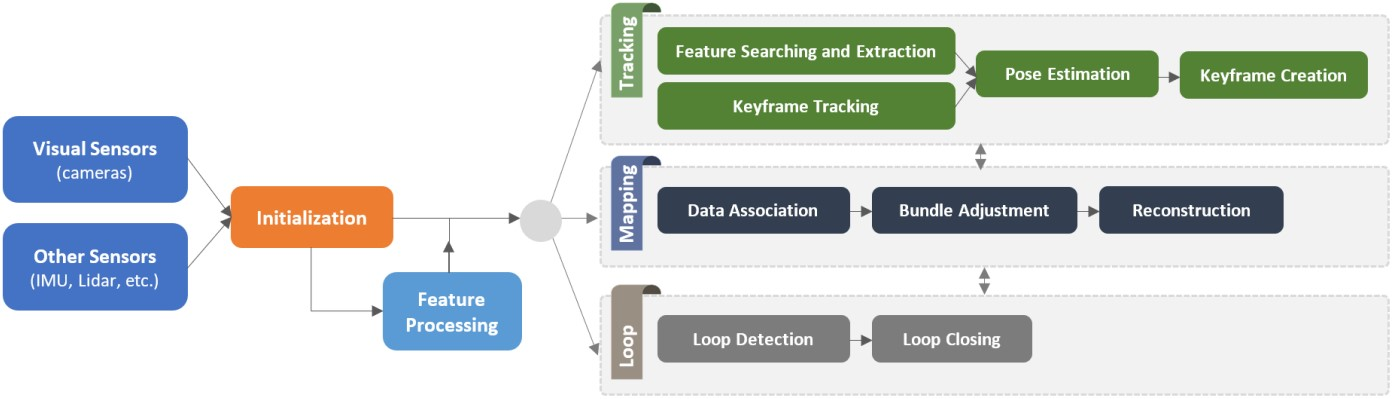
\includegraphics[ width=1\textwidth ]{VSLAM}
    \caption{Funktionsweise des Visual SLAM\label{fig:VSLAM}}\par
\end{figure}

Die Abbilung \ref{fig:VSLAM} zeigt die einzelnen Schritte des Visual SLAM. SLAM kann in Bezug auf dessen Funktionsweise in ein Frontend und ein Backend unterteilt werden. Das Frontend umfasst die Schätzung der Kameraposition und der 3D-Struktur der Szene (Tracking, siehe Abbildung \ref{fig:VSLAM}), während das Backend die Optimierung der Schätzungen und die Erstellung einer konsistenten Karte übernimmt (Mapping, siehe Abbildung \ref{fig:VSLAM}). Die einzelnen Schritte des vSLAM werden im Folgenden näher erläutert.

\subsection{Feature Detection}

Bei der Feature Detection werden Feature-Punkte in Bildern identifiziert. Ein Feature-Punkt (Merkmal) ist ein charakteristischer Punkt in einem Bild, der durch seine einzigartige Struktur oder Helligkeitsverteilung hervorsticht. Ein Feature-Punkt kann beispielsweise ein Eckpunkt, ein Kantenpunkt oder ein Texturpunkt sein. Feature-Punkte bestehen aus einem Key Point, also einem zweidimensionalen Punkt im Bild, und einem Descriptor. 

Der Descriptor entspricht einer numerischen Beschreibung des erkannten Merkmals, um sie über mehrere Bilder hinweg vergleichbar zu machen. Diese Deskriptoren bestehen in der Regel aus Vektoren, die die verschiedene Charakteristiken, wie der Helligkeitsverteilung, um den jeweiligen Feature-Punkt erfassen. Korrespondierende Feature Punkte werden anhand der Ähnlichkeiten der Deskriptoren im Vektorraum gefunden.

Es gibt verschiedene Algorithmen, die für das Erkennen und Nachverfolgen von Feature-Punkten verwendet werden können, wie z. B. SIFT (Scale-Invariant Feature Transform), SURF (Speeded-Up Robust Features) oder ORB (Oriented FAST and Rotated BRIEF). Die folgende Tabelle vergleicht die Geschwindigkeit der erwähnten Algorithmen bei einer Extraktion von 1000 Feature-Punkten aus dem gleichen Bild:

\begin{center}
    \begin{tabular}{ |c|c| } 
        \hline
        Algorithmus & Geschwindigkeit (ms) \\
        \hline
        SIFT & 5228.7 \\
        SURF & 217.3 \\
        ORB & 15.3 \\
        \hline
    \end{tabular}
\end{center}

Aufgrund der Echtzeit-Anforderung in AR-Anwendungen wird neben der Robustheit, vor allem die Geschwindigkeit der Algorithmen betrachtet. ORB stellt hierbei eine gute Balance zwischen Geschwindigkeit und Robustheit dar und wird daher häufig in AR-Anwendungen eingesetzt. Aus diesem Grund wird ORB im folgenden Abschnitt näher erläutert.

Oriented FAST and Rotated BRIEF (ORB) setzt sich aus zwei Komponenten zusammen: FAST (Features from Accelerated Segment Test) und BRIEF (Binary Robust Independent Elementary Features). Der FAST-Algorithmus identifiziert Punkte mit starken Helligkeitsänderungen in den Grauwerten, indem er benachbarte Pixel in einem Kreis um den zu prüfenden Pixel vergleicht. 

Die Abbildung \ref{fig:FAST} zeigt die Funktionsweise des FAST-Algorithmus. Zunächst wird ein Pixel \( p \) mit einem Helligkeitswert \( I_p \) ausgewählt. Ausgehend von diesem Pixel werden die Helligkeitswerte der 16 benachbarte Pixel \( p \) in einem Kreis mit einem Radius von 3 verglichen. Übersteigt die Anzahl der aufeinander folgenden, signifikant helleren oder dunkleren Pixel einen bestimmten Schwellenwert \( N \), wird \( p \) als Feature identifiziert. Diese Schritte werden für alle Pixel im Bild wiederholt, um alle Feature-Punkte zu identifizieren. Der Algorithmus kann optimiert werden, indem zunächst die Nachbarpixel 1, 5, 9, und 13 (siehe Abbildung \ref{fig:FAST}) betrachtet werden. Falls drei der vier Pixel heller oder dunkler sind als \( I_p \), kann es sich um einen potenziellen Feature-Punkt handeln.

\begin{figure}
    \centering
    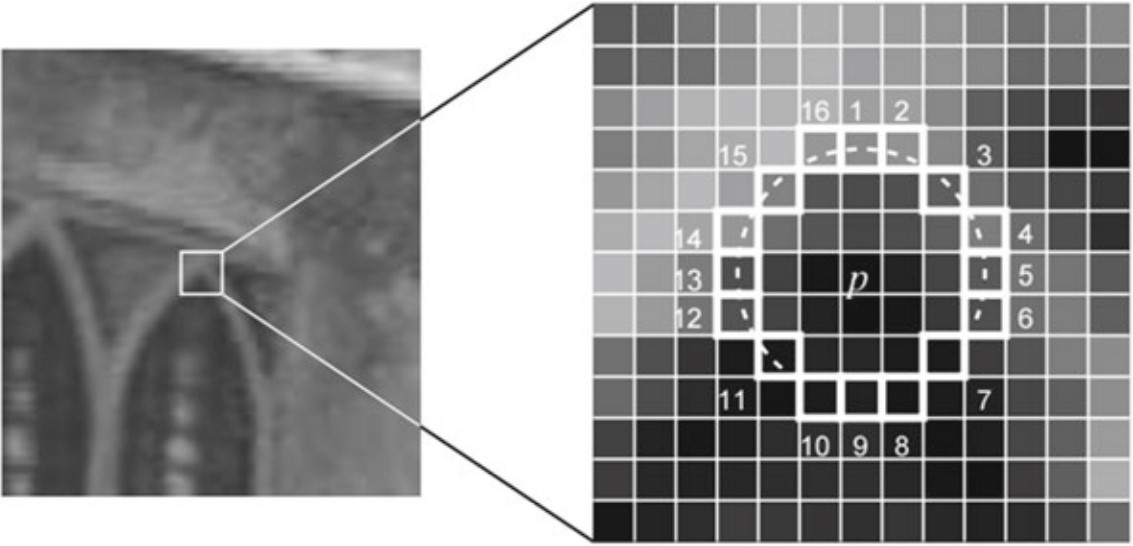
\includegraphics[ width=.5\textwidth ]{FAST}
    \caption{FAST-Feature-Punkte\label{fig:FAST}}\par
\end{figure}

Zusätzlich zu den erkannten Feature-Punkten berechnet ORB Rotations- bzw. Richtungsinformationen für jedes Feature. Dazu wird ein sogenannter Zentroid berechnet, der den Grauwert des Bildblocks in der Nähe des Feature-Punkts als Schwerpunkt verwendet. Diese Zentroide werden wie folgt berechnet:

Zunächst wird das Moment \( m_{pq} \) im Bildblock \( B \) berechnet, wobei \( p \) und \( q \) entweder 0 oder 1 sind:

\begin{equation}
    m_{pq} = \sum_{x,y \in B} x^p y^q I(x, y)
\end{equation}

\begin{tcolorbox}[colback=THAi-Blue!20!white, colframe=THAi-Blue]
    Momente sind gewichtete Mittelwerte der Pixelintensitäten und dienen in der Bildverarbeitung zur Objektbeschreibung nach der Segmentierung. Sie ermöglichen die Bestimmung von Fläche, Schwerpunkt und Ausrichtung eines Objekts.
\end{tcolorbox}

Mithilfe der Momente kann nun der inhaltsbasierte Schwerpunkt \( C \) (auch ,,centroid'' genannt) des Bildblocks berechnet werden:

\begin{equation}
C = 
\left(
\frac{m_{10}}{m_{00}}, \\
\frac{m_{01}}{m_{00}}
\right)
\end{equation}

Schließlich wird die Orientierung des Features bestimmt, die durch den Vektor \( \overrightarrow{OC} \) vom geometrischen Zentrum des Bildblocks \( O \) zum Zentroiden \( C \) definiert ist und durch den Winkel \( \theta \) beschrieben wird. Die Berechnung kann verkürzt werden, indem der Tangens des Winkels \( \theta \) durch das Verhältnis der Momente \( m_{01} \) und \( m_{10} \) berechnet wird:

\begin{equation}
    \theta = \arctan \left( \frac{m_{01}}{m_{10}} \right)
\end{equation}

Nachdem die Feature-Punkte erkannt wurden, werden die Deskriptoren für jedes Feature berechnet. Der BRIEF-Algorithmus erstellt binäre Deskriptoren, die die Helligkeitsverteilung um den Feature-Punkt beschreiben. Dabei werden zufällige Paare von Pixeln um den Feature-Punkt ausgewählt und verglichen. Die resultierenden binären Werte werden in einem 128-bit Vektor gespeichert und bilden den Deskriptor für das Feature.

Die verbesserte Implementierung des FAST- und BRIEF-Algorithmus in ORB ermöglicht eine schnelle und robuste Merkmalsextraktion, die in Echtzeit auf mobilen Geräten ausgeführt werden kann. Die Features sind invariant gegenüber Rotationen und Skalierungen und eignen sich daher gut für das Feature-Matching in AR-Anwendungen. ORB wird daher häufig in AR-Anwendungen eingesetzt, um Feature-Punkte zu erkennen und zu verfolgen.

Neben klassischen Verfahren wie ORB gewinnen Deep-Learning-Modelle zunehmend an Bedeutung für das Feature Matching. Besonders Convolutional Neural Networks (CNNs) und Transformer-Modelle liefern vielversprechende Ergebnisse. Ein Beispiel hierfür ist XFeat (Accelerated Features), ein optimiertes neuronales Netzwerk, das die Merkmalsextraktion beschleunigt. Auch OmniGlue, eine Kombination aus CNNs und Transformer-Modellen, setzt neue Maßstäbe in der robusten und anpassungsfähigen Feature-Matching-Strategie. Diese modernen Ansätze bieten oft eine höhere Genauigkeit und Stabilität, insbesondere in komplexen Szenen oder bei stark variierenden Lichtverhältnissen.

\subsection{Feature Matching}

Das Feature Matching ist ein wichtiger Schritt im visual SLAM, bei dem die Korrespondenzen zwischen den Feature-Punkten in aufeinanderfolgenden Bildern gefunden werden. Dies ermöglicht die spätere Bestimmung der Kamerabewegung. 

Die Feature-Matching-Algorithmen vergleichen die Deskriptoren der Feature-Punkte und bestimmen die Ähnlichkeiten zwischen den Merkmalen. Korrespondierende Feature-Punkte werden anhand der Ähnlichkeiten der Deskriptoren mithilfe von Distanzmaßen, wie dem euklidischen Abstand oder dem Hamming-Abstand, gefunden. 

Da die Anzahl der Feature-Punkte in den Bildern hoch sein kann, ist es wichtig, effiziente Algorithmen für das Feature Matching zu verwenden. Ein bekannter Algorithmus ist der FLANN-Algorithmus (Fast Library for Approximate Nearest Neighbors), der eine effiziente Suche nach den nächsten Nachbarn in großen Datensätzen ermöglicht. Der FLANN-Algorithmus verwendet k-d-Bäume oder andere Datenstrukturen, um die Suche nach den nächsten Nachbarn zu beschleunigen. 

\subsection{Pose Estimation}

Die Schätzung der Kameraposition (Pose Estimation) ist ein essenzieller Schritt in der SLAM-Pipeline. Sie liefert die Grundlage für die Rekonstruktion der dreidimensionalen Szene und die Bestimmung der extrinsischen Kameraparameter. Die Pose Estimation basiert auf der Triangulation, bei der die dreidimensionale Position eines Punktes im Raum anhand der korrespondierenden Punkte in zwei oder mehr Bildern bestimmt wird.

Dazu wird zunächst identifiziert, wie sich die Kamera zwischen zwei oder mehreren Bildern bewegt hat. Die Epipolargeometrie beschreibt die Beziehung zwischen den Bildern und ermöglicht die Bestimmung der Kameraposition.  Das Ziel ist es, eine sogenannte Essential Matrix zu berechnen, die die Rotation \( R \) und Translation \( t \) der Kamera zwischen den Bildern beschreibt.

Dazu betrachten wir die Situation in Abbildung \ref{fig:Epipolar} mit zwei Bildern \( I_1 \) und \( I_2 \) und den korrespondierenden Punkten \( p_1 \) und \( p_2 \). Die Kamerapositionen \( C_1 \) und \( C_2 \) sind ebenfalls dargestellt. 

\begin{figure}
    \centering
    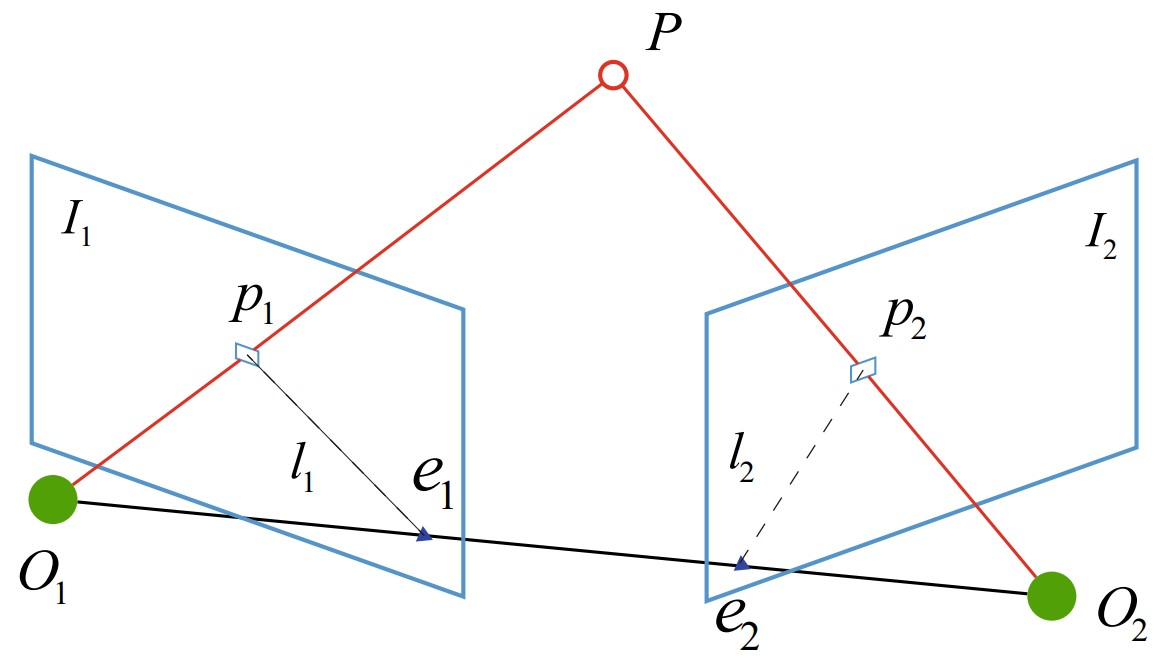
\includegraphics[ width=.5\textwidth ]{Epipolar}
    \caption{Situation der Epipolargeometrie bei zwei Bildern\label{fig:Epipolar}}\par
\end{figure}

Die epipolare Bedingung beschreibt, dass die Kamerapositionen \( C_1 \) und \( C_2 \) zusammen mit dem Punkt \( P \), der dem Schnittpunkt der Linien \( \overrightarrow{O_1p_1} \) und \( \overrightarrow{O_2p_2} \) entspricht, auf einer Ebene liegen. Diese Bedingung kann durch die folgende Gleichung ausgedrückt werden:

\begin{equation}
    x_2^T t \times R x_1 = 0
\end{equation}

Hierbei entsprechen \( x_1 \) und \( x_2 \) den homogenen Koordinaten der korrespondierenden Punkte \( p_1 \) und \( p_2 \) in den Bildern \( I_1 \) und \( I_2 \). Die Essential Matrix \( E \) wird nun wie folgt definiert:

\begin{equation}
    E = t \times R
\end{equation}

Diese Matrix entspricht einer 3x3-Matrix mit neun unbekannten Variablen. Die Essential Matrix kann mithilfe des Eight-Point-Algorithmus geschätzt werden, der die epipolare Bedingung für mindestens acht korrespondierende Punkte in den Bildern verwendet. Dazu wird ein Lineares Gleichungssystem wie folgt aufgestellt: 

\begin{equation}
    \begin{pmatrix}
        u_2^1 u_1^1 & u_2^1 v_1^1 & u_2^1 & v_2^1 u_1^1 & v_2^1 v_1^1 & v_2^1 & u_1^1 & v_1^1 & 1 \\
        u_2^2 u_1^2 & u_2^2 v_1^2 & u_2^2 & v_2^2 u_1^2 & v_2^2 v_1^2 & v_2^2 & u_1^2 & v_1^2 & 1 \\
        \vdots & \vdots & \vdots & \vdots & \vdots & \vdots & \vdots & \vdots & \vdots \\
        u_2^8 u_1^8 & u_2^8 v_1^8 & u_2^8 & v_2^8 u_1^8 & v_2^8 v_1^8 & v_2^8 & u_1^8 & v_1^8 & 1 
    \end{pmatrix}
    \begin{pmatrix}
        e_1 \\ e_2 \\ e_3 \\ e_4 \\ e_5 \\ e_6 \\ e_7 \\ e_8 \\ e_9
    \end{pmatrix}
    = 0
\end{equation}

Die Essential Matrix \( E \) kann durch die Singulärwertzerlegung (SVD) in die Rotationsmatrix \( R \) und die Translationsmatrix \( t \) zerlegt werden. Die genaue Beschreibung dieser Zerlegung ist kein Bestandteil dieses Kapitels. Stattdessen wird auf weiterführende Literatur verwiesen.

Wichtig ist, dass die Zerlegung der Essential Matrix vier mögliche Lösungen liefert, die durch die Wahl der korrekten Lösung bestimmt werden müssen. Die Abbildung \ref{fig:SVD} zeigt ein Beispiel für die vier möglichen Lösungen der Zerlegung der Essential Matrix. In diesem Fall kann die korrekte Lösung durch die Überprüfung der positiven Parallaxe bestimmt werden, die angibt, ob die Punkte vor oder hinter der Kamera liegen. Die korrekte Lösung entspricht derjenigen, bei der die meisten Punkte vor der Kamera liegen. Das Ergebnis der Zerlegung ist die Rotation \( R \) und die Translation \( t \), die die Bewegung der Kamera zwischen den Bildern beschreiben.

\begin{figure}
    \centering
    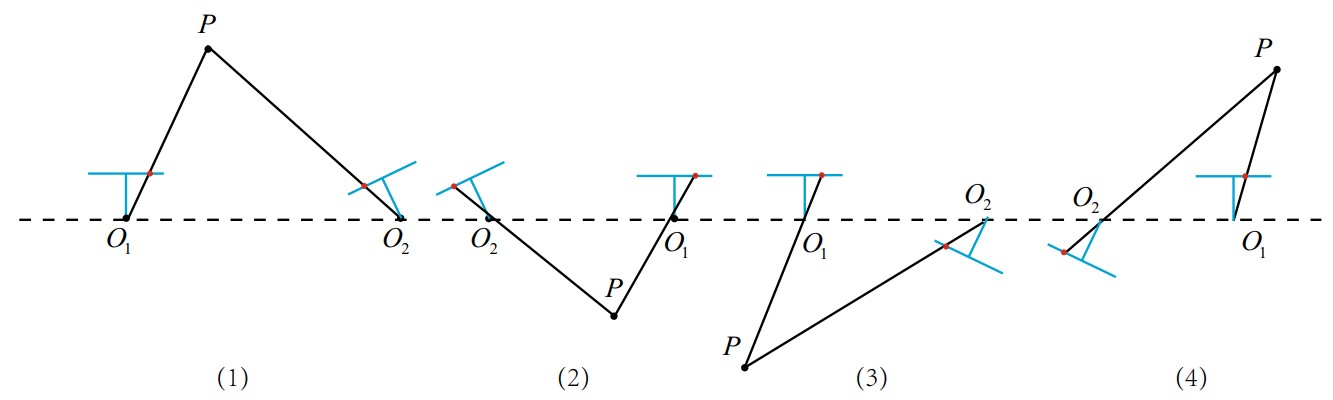
\includegraphics[ width=1\textwidth ]{SVD}
    \caption{Zerlegung der Essential Matrix\label{fig:SVD}}\par
\end{figure}

Offensichtlich können wir allein von der Bewegung der Kamera zwischen zwei Bildern nicht direkt auf die Position der Kamera im Weltkoordinatensystem schließen. Dazu wird meistens bei der Initialisierung des AR-Systems das Weltkoordinatensystem auf die Position der Kamera im ersten Bild gelegt. Die Position der Kamera im Weltkoordinatensystem wird dann durch die Bewegung der Kamera zwischen den Bildern bestimmt.

\subsection{Triangulation}

Bei der Triangulation werden die kartesischen Koordinaten eines Feature-Punktes in zwei oder mehr Bildern im Raum bestimmt. Dies führt zur Extraktion von Tiefeninformationen aus den vohanden Bildern und ermöglicht die Rekonstruktion der dreidimensionalen Struktur der Szene. 

Die Abbildung \ref{fig:Triangulation} zeigt die Triangulation eines Punktes im dreidimensionalen Raum anhand von zwei Bildern. Die Kamerapositionen \( O_1 \) und \( O_2 \) sowie die korrespondierenden Punkte \( p_1 \) und \( p_2 \) sind dargestellt. Der Punkt \( P \) entspricht dem gesuchten Feature-Punkt im Raum. In einer idealen Welt entspricht \( P \) dem Schnittpunkt der Strahlen \( \overrightarrow{O_1p_1} \) und \( \overrightarrow{O_2p_2} \). Aufgrund von Rauschen und Ungenauigkeiten in den Bildern ist die exakte Bestimmung des Punktes durch die Berechnung des Schnittpunktes meist nicht möglich. Stattdessen wird der gesuchte Punkt durch die Minimierung der quadratischen Abstände zwischen den Strahlen und dem Punkt berechnet. Der gesuchte Punkt \( P \) ist derjenige, der sich im minimalen Abstand zu allen Strahlen befindet (siehe Abbildung \ref{fig:Triangulation}).

\begin{figure}
    \centering
    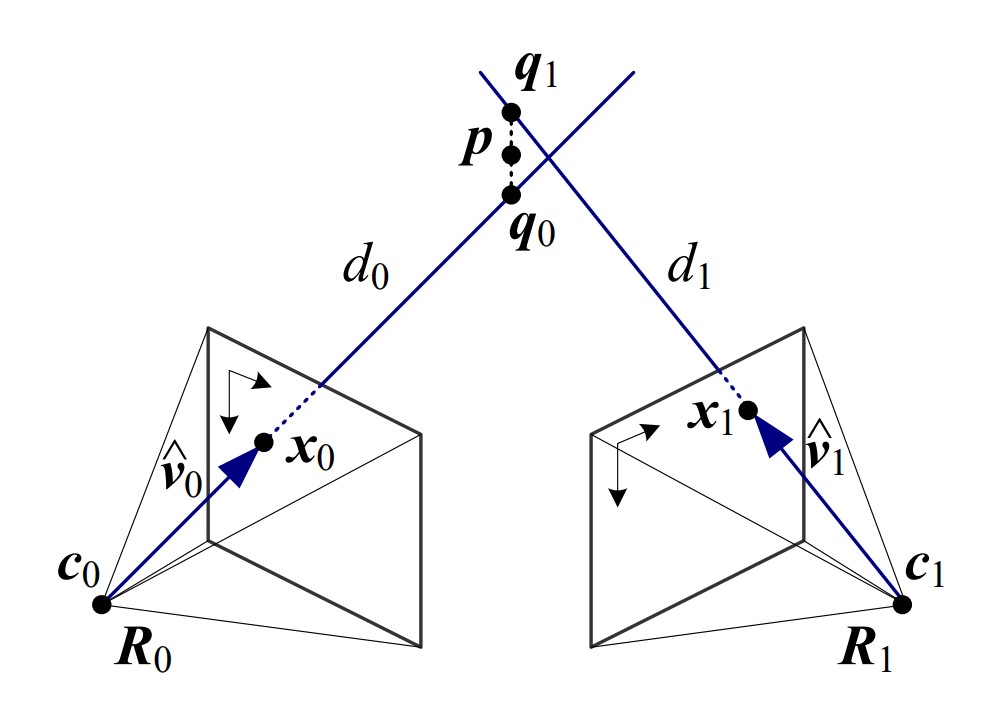
\includegraphics[width=.5\textwidth]{Triangulation}
    \caption{Dreidimensionale Triangulation mit zwei Bildern\label{fig:Triangulation}}\par
\end{figure}

Das Ergebnis der Triangulation verschiedener Feature-Punkte über mehrere Bilder ergibt eine sogenannte Punktwolke (Point Cloud), die die 3D-Struktur der Szene abbildet. Diese Punktwolke kann anschließend weiterverarbeitet werden, um ein detailliertes 3D-Modell der Szene zu erstellen. Ein wichtiger Schritt in dieser Weiterverarbeitung ist die Oberflächenrekonstruktion (Plane Detection), bei der die Punktwolke in Flächen unterteilt wird, um die Oberflächen von Objekten im Raum zu bestimmen. Zur Durchführung der Oberflächenrekonstruktion wird häufig der RANSAC-Algorithmus (Random Sample Consensus) eingesetzt. Dieser Algorithmus erkennt Ausreißer in den Daten und schätzt die Flächen anhand der verbleibenden, konsistenten Punkte.

\begin{figure}
    \centering
    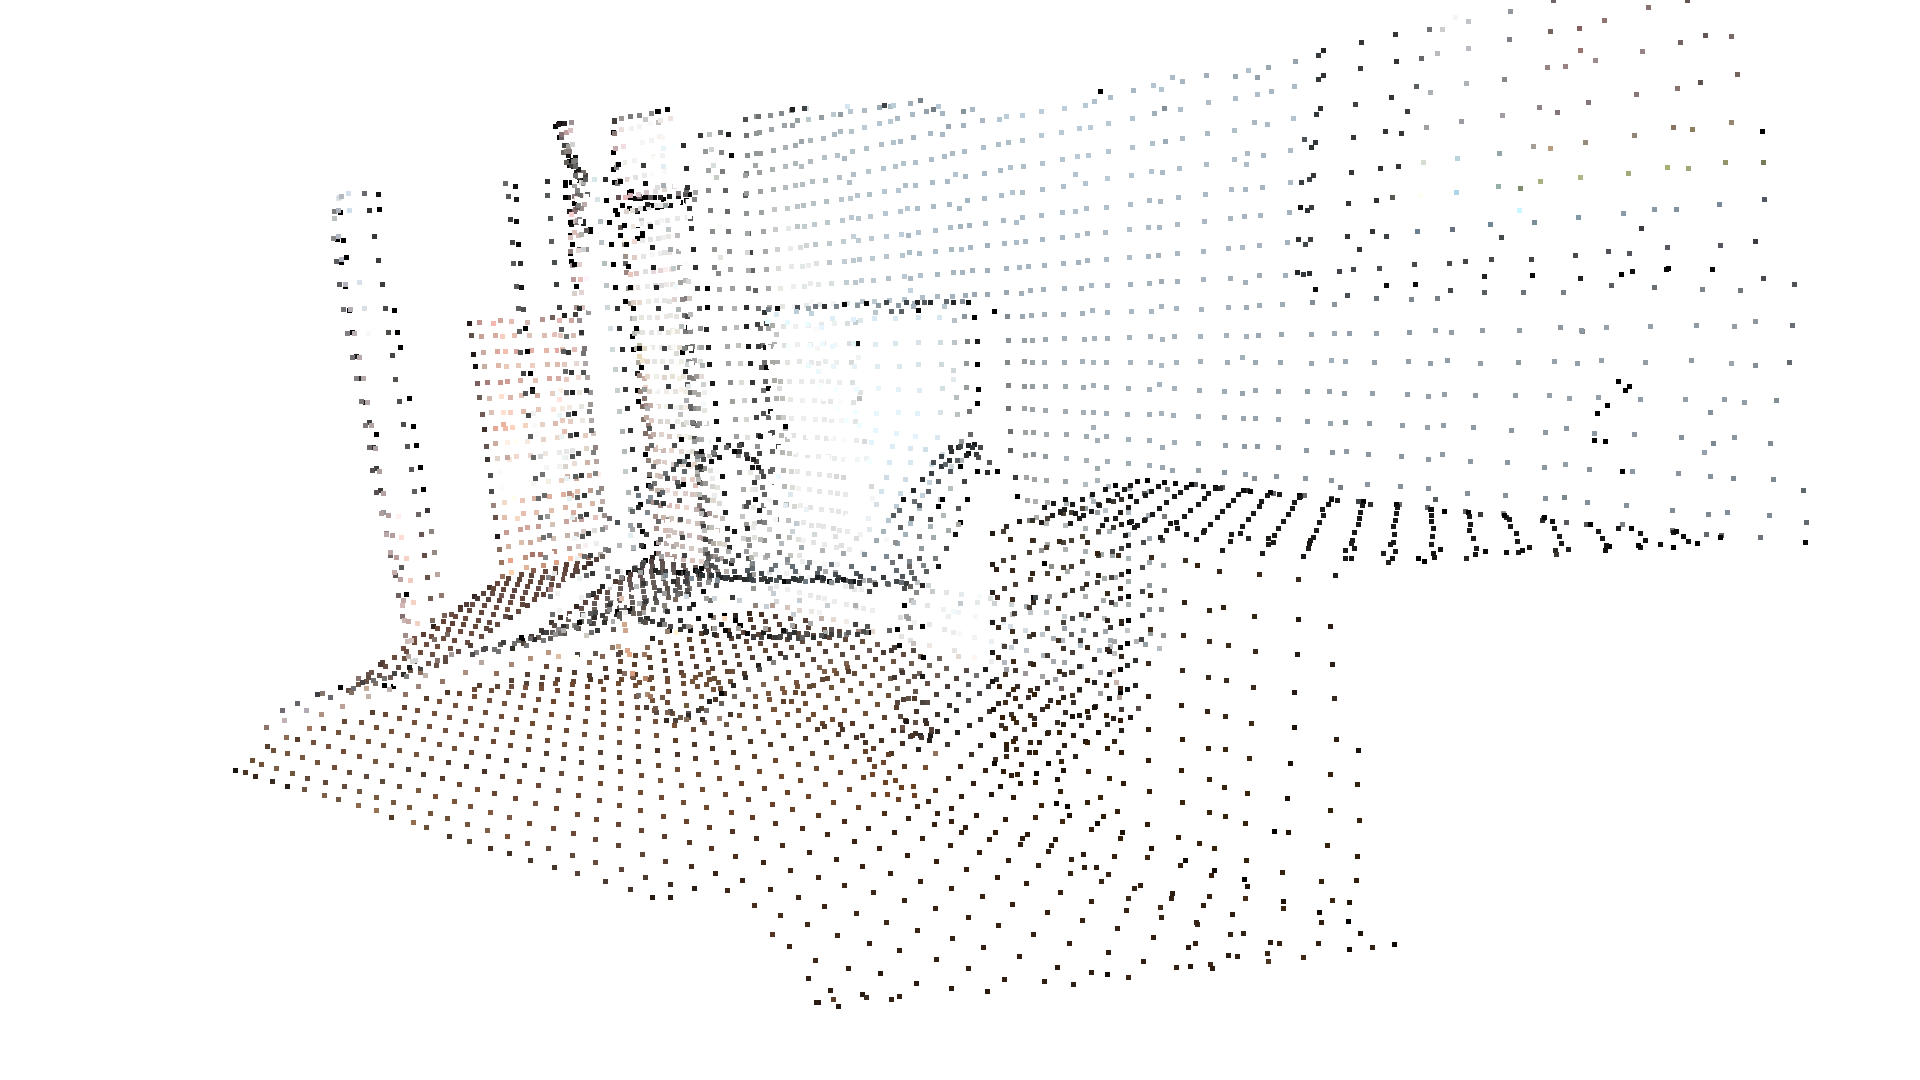
\includegraphics[ width=.5\textwidth ]{PointCloud}
    \caption{Beispiel einer dreidimensionalen Point-Cloud-Rekonstruktion\label{fig:PointCloud}}\par
\end{figure}

\subsection{Bundle Adjustment}

Aufgrund der Ungenauigkeiten in den Bildern und der dadurch entstehenden ungenauen Schätzungen der Kamerapositionen und Feature-Punkte im Weltkoordinatensystem ist es notwendig, die gesamte Szene zu optimieren, um eine konsistente und präzise Rekonstruktion zu erhalten. 

In der computergestützten Photogrammetrie sowie in SLAM-Systemen (Simultaneous Localization and Mapping) ist die \emph{Bundle Adjustment} (BA) eine zentrale Methode zur gleichzeitigen Optimierung von Kameraposen und 3D-Punktwolken. Ziel des Verfahrens ist es, den sogenannten Reprojektionsfehler zu minimieren, also die Differenz zwischen den in den Bildern gemessenen 2D-Punkten und den Projektionen der rekonstruierbaren 3D-Punkte zu reduzieren. 

\begin{figure}
    \centering
    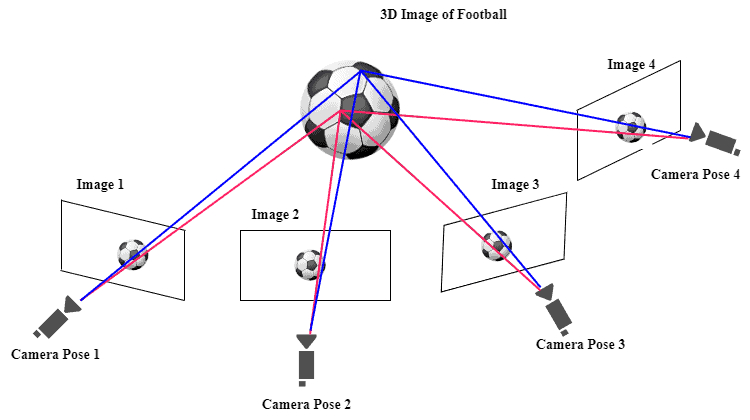
\includegraphics[ width=.8\textwidth ]{BundleAdjustment}
    \caption{Beispiel einer Situation mit Reprojektionsfehler\label{fig:BA}}\par
\end{figure}

Dieser, in Abbildung \ref{fig:BA} dargestellte, Reprojektionsfehler tritt aufgrund der Ungenauigkeiten bei der Triangulation und der Schätzung der Kamerapositionen auf. Um diesen Fehler zu minimieren, wird zunächst der triangulierte Punkt im Weltkoordinatensystem zurück in das Kamerabild projiziert. Dazu werden sowohl die extrinsische Parameter als auch die intrinschen Parameter der Kamera (siehe Kapitel \ref{Kalibrierung}) wie folgt verwendet:
\begin{equation}
    P' = Rp+t = [X', Y', Z']^T
\end{equation}

Anschließend wird der Punkt \( P' \) in die normalisierte Bildebene projiziert:
\begin{equation}
    P_c = [u_c, v_c, 1]^T = \frac{1}{Z'}[X', Y', Z']^T = [X'/Z', Y'/Z', 1]^T
\end{equation}

Nun können Verzeichnungen der Linse einbezogen werden:
\begin{equation}
    \begin{aligned}
        u'_c &= u_c(1 + k_1r^2 + k_2r^4 + k_3r^6) \\
        v'_c &= v_c(1 + k_1r^2 + k_2r^4 + k_3r^6)
    \end{aligned}
\end{equation}

Die Anwendung der intrinsischen Parameter liefert die Pixelkoordinaten des reprojizierten Punktes im Bild:
\begin{equation}
    \begin{aligned}
        u &= f_xu'_c + c_x \\
        v &= f_yv'_c + c_y
    \end{aligned}
\end{equation}

Der Reprojektionsfehler kann nun wie folgt berechnet werden:
\begin{equation}
    e = z - h(T,p)
\end{equation}

Wobei \( z \) der beobachtete 2D-Punkte und \( h(T,p) \) der reprojizierte 2D-Punkt ist. Der Reprojektionsfehler wird dann über alle Merkmale summiert:
\begin{equation}
    \frac{1}{2} \sum_{i=1}^{m} \sum_{j=1}^{n} \| e_{ij} \|^2 = \frac{1}{2} \sum_{i=1}^{m} \sum_{j=1}^{n} \| z_{ij} - h(T_i, p_j) \|^2
\end{equation}

Bei dieser Summe handelt es sich um ein nichtlineares Optimierungsproblem, das mithilfe von numerischen Optimierungsmethoden gelöst werden kann. Ein bekanntes Verfahren zur Lösung des Bundle Adjustment ist das Levenberg-Marquardt-Verfahren, das eine Kombination aus dem Gauss-Newton-Verfahren und der Methode der kleinsten Quadrate darstellt.

\subsection{Loop Closure}

Während das Bundle Adjustment die Optimierung der Kamerapositionen und Feature-Punkte über aufeinanderfolgende Bilder ermöglicht, ist es nicht in der Lage, Fehler zu korrigieren, die durch wiederkehrende Strukturen oder Schleifen in der Szene entstehen. Diese Fehler entstehen durch die Akkumulation von Ungenauigkeiten in der Schätzung der Kamerapositionen und Feature-Punkte über mehrere Bilder hinweg. 

Die Loop Closure Detection ist ein Verfahren zur Erkennung und Korrektur von Fehlern in der Kamerapositionsschätzung. Dabei werden Schleifen in der Szene erkannt und die Kamerapositionen entsprechend korrigiert. Anstatt die einzelnen Deskriptoren der Feature-Punkte mehrere Bilder zu vergleichen, werden die Bilder als Ganzes betrachtet und anhand ihrer visuellen Ähnlichkeit miteinander verglichen.

Dazu wird das sogenannte Bag-of-Words-Modell eingesett. Dieses Modell bestimmt die Ähnlichkeit von Bildern anhand von visuellen Wörtern. Dazu wird zunächst ein Wörterbuch mit fixer Größe erstellt, das die häufigsten Wörter in den Bildern repräsentiert. Ein Wort kann dabei als eine Menge benachbarter Merkmalspunkte angesehen werden. Anschließend werden die Bilder mithilfe des Wörterbuches in eine Vektorform kodiert. Ein Bild \( A \) könnte somit wie folgt kodiert werden:
\begin{equation}
    A = [1, 1, 0]^T
\end{equation}

Wobei die Länge des Vektoren die Anzahl der Wörter im Wörterbuch entrspricht und der Vektor das Vorhandensein der visuellen Wörter \( w_1 \) und \( w_2 \) und die Abwesenheit von \( w_3 \) in einem Bild repräsentiert. Eine andere Möglichkeit ist die Kodierung der Häufigkeiten der visuellen Wörter in einem Bild:
\begin{equation}
    B = [2, 1, 0]^T
\end{equation}

Hier repräsentiert der Vektor \( B \) wie oft die visuellen Wörter \( w_1 \), \( w_2 \), \( w_3 \) in einem Bild vorkommen. Die Ähnlichkeit von Bildern kann dann mithilfe von Distanzmaßen, wie dem euklidischen Abstand oder dem Kosinus-Ähnlichkeitsmaß, bestimmt werden. Bilder mit ähnlichen Vektorkodierungen werden als ähnlich betrachtet und können als mögliche Schleifen in der Szene erkannt werden. 

Eine weitaus elegantere Lösung der Loop Closure Detection ist die Bestimmung des Wörtebuches mithilfe eines k-d-Baums. Dieser Baum weist eine Tiefe von \( d \) auf und besitzt \( k \) Verzweigungen am Wurzelknoten. Mithilfe des k-means Clustering wird das Wörterbuch erstellt, indem die Merkmalspunkte der betrachteten Bilder in \( k \) Cluster unterteilt werden. Diese Cluster entsprechen der ersten Ebene des k-d-Baums. Anschließend werden die Cluster in weitere Cluster unterteilt, bis die gewünschte Tiefe \( d \) erreicht ist.


\begin{tcolorbox}[colback=THAi-Blue!20!white, colframe=THAi-Blue]
    Clustering ist ein Verfahren des unüberwachten Lernens, bei dem ähnliche Objekte in Gruppen (Cluster) zusammengefasst werden. Ziel ist es, Muster oder Strukturen in unklassifizierten Daten zu erkennen. 
\end{tcolorbox}




Die Kamera- und Feature-Punktschätzungen können dann entsprechend angepass werden, um den akkumulierten Fehler zu eliminieren und eine konsistente Rekonstruktion der Szene zu gewährleisten.



\section{Scene Understanding}

Die Scene Understanding bezeichnet die Fähigkeit eines Systems, die Umgebung zu interpretieren und zu verstehen. Ein wichtiger Bestandteil des Scene Understanding ist die semantische Segmentierung, bei der die Pixel eines Bildes in verschiedene Klassen eingeteilt werden. Diese Klassen können beispielsweise Objekte, Personen oder Hintergründe sein. Dadurch lassen sich einzelne Elemente in der Szene, wie Wände, Decken oder Möbel, identifizieren und voneinander unterscheiden. Die semantische Segmentierung ist ein wichtiger Schritt in der AR, da sie die Grundlage für die Interaktion zwischen virtuellen und realen Objekten bildet.



\section{Technische Limitationen}

Viele der gängigen Algorithmen zur Feature-Erkennung und -Verfolgung, wie SIFT oder ORB, verlassen sich stark auf die visuelle Qualität der Eingabebilder. In Umgebungen mit schlechten Lichtverhältnissen (z. B. bei schwacher Beleuchtung, direkter Sonneneinstrahlung oder Nachtaufnahmen) wird die Fähigkeit der Algorithmen zur präzisen Merkmalserkennung und -verfolgung beeinträchtigt. Dies kann zu fehlerhaften Schätzungen der Kameraposition oder der 3D-Rekonstruktion führen.

Ein weiteres Problem tritt auf, wenn sich die Umgebung schnell verändert, etwa bei Bewegungen von Objekten, plötzlichen Änderungen der Szene oder in dynamischen Umgebungen. In solchen Fällen können Feature-Punkte in den Bildern verschwinden oder durch neue, nicht korrespondierende Punkte ersetzt werden, was die Stabilität der Berechnungen negativ beeinflusst.

Auch LiDAR-basierte Systeme sind von technischen Einschränkungen betroffen. Zum einen haben LiDAR-Sensoren eine begrenzte Reichweite, die oft auf wenige Meter beschränkt ist, wodurch sie nicht für alle Anwendungen geeignet sind, insbesondere bei großen Distanzen oder in weiten offenen Bereichen.

Zudem sind LiDAR-Sensoren in der Regel teuer und daher nur vereinzelt in Smartphones verbaut. LiDAR-basierte Systeme sind vor allem in spezialisierten Bereichen wie der Automobilindustrie oder der Robotik weit verbreitet, aber in konsumerorientierten Geräten noch eher selten.